\documentclass[addpoints]{exam}
\usepackage{preamble}
\sisetup{group-separator = {,}}

\pagestyle{headandfoot}
\runningheadrule

\usepackage{etoolbox}

\providetoggle{printlines}
\settoggle{printlines}{false}

\providetoggle{printstars}
\settoggle{printstars}{false}

% \firstpagefooter{Access for free at \href{https://openstax.org/books/astronomy-2e/pages/1-introduction}{https://openstax.org/books/astronomy-2e/pages/1-introduction}}{}{}
% \runningfooter{Access for free at \href{https://openstax.org/books/astronomy-2e/pages/1-introduction}{https://openstax.org/books/astronomy-2e/pages/1-introduction}}{}{}

\firstpageheader{Astronomy}{Study Guide for Final Exam: Semester 1}{December 2022}


\CorrectChoiceEmphasis{\color{red}\bfseries}
\SolutionEmphasis{\color{red}}
\printanswers

\begin{document}
\begin{questions}

% \question
% What is the tilt of Earth's axis relative to its orbit around the Sun?

% \begin{choices}
%     \correctchoice \SI{23.5}{\degree}
%     \choice \SI{45}{\degree}
%     \choice \SI{21}{\degree}
%     \choice \SI{0}{\degree}
% \end{choices}

\question
Here in Texas, we live in Earth's \fillin\ hemisphere.

\begin{choices}
    \choice Southern
    \correctchoice Northern
    \choice Eastern
    \choice Western
\end{choices}

\question
Why are the summer months in Texas so hot?

\begin{choices}
    \choice Earth is much closer to the Sun in the summer
    \correctchoice the northern hemisphere is tilted towards the Sun, absorbing more daily sunlight
    \choice people are more active, causing body heat to dissipate throughout the environment
    \choice during the summer the Sun becomes hotter and brighter for a few months
\end{choices}

% \question
% The figures below represent direct (a) and indirect (b) sunlight. Which figure could represent the Antarctica (latitude \SI{80}{\degree}\,S) June?

% \question 
% The figures below represent direct (a) and indirect (b) sunlight. Which figure could represent a city at latitude \SI{56}{\degree}\,N in June?

% \question
% The figures below represent direct (a) and indirect (b) sunlight. Which figure could represent South Africa (latitude \SI{30}{\degree}\,S) in December?

% \begin{figure}[h!]
%     \centering
%     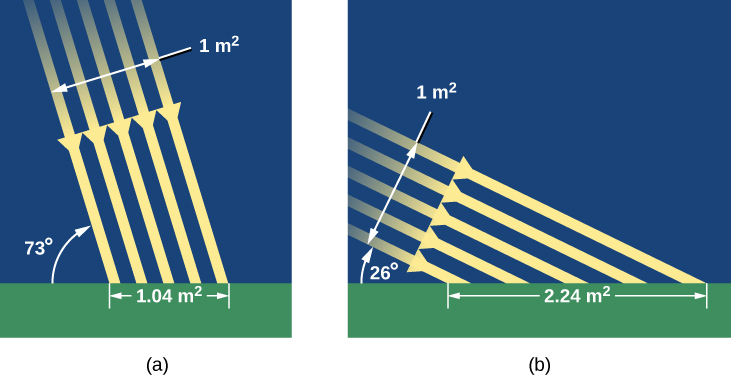
\includegraphics{Figures/Figure4.6.jpg}
% \end{figure}

% \clearpage

% \question
% Which of the following is NOT a reason why summer months are hotter in the Northern Hemisphere?

% \begin{choices}
%     \choice Sunlight strikes northern countries more directly
%     \correctchoice Earth is 3\% closer to the Sun on June 21
%     \choice The Sun is visible for more time
%     \choice Earth's southern hemisphere is tilted away from the Sun
% \end{choices}

\question
Which astronomical event is depicted in the figure below?

\begin{minipage}{0.45\textwidth}
    \centering
    \begin{choices}
    \choice Winter solstice (December 21)
    \choice Spring Equinox (March 21)
    \correctchoice Summer solstice (June 21)
    \choice Fall Equinox\\ (September 21)
    \end{choices}
\end{minipage}%
\begin{minipage}{0.5\textwidth}
    \centering
    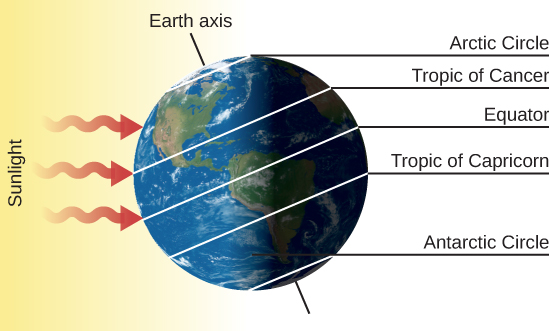
\includegraphics[width=2.5in]{Figures/Figure4.8.jpg}
\end{minipage}
\vspace{1em}

% \question
% Which astronomical event is depicted in the figure below?

% \begin{minipage}{0.45\textwidth}
%     \centering
%     \begin{choices}
%     \choice Spring Equinox\\ (March 21)
%     \choice Fall Equinox\\ (September 21)
%     \choice Summer Solstice\\ (June 21)
%     \correctchoice Winter Solstice\\ (December 21)
%     \end{choices}
% \end{minipage}%
% \begin{minipage}{0.5\textwidth}
%     \centering
%     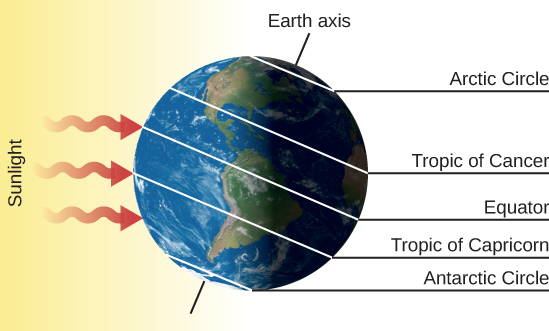
\includegraphics[width=2.5in]{Figures/Figure4.9.jpg}
% \end{minipage}
% \vspace{1em}

% \question
% The Tropic of Cancer is at latitude \fillin[][1cm]\ .

% \begin{choices}
%     \correctchoice \SI{23}{\degree N}
%     \choice \SI{0}{\degree} (Equator)
%     \choice \SI{23}{\degree S}
%     \choice \SI{45}{\degree W}
% \end{choices}

% \question
% If you travel to a place on the Tropic of Cancer (e.g., Hawaii) on the summer solstice, you'll observe that the Sun at noon \ldots

% \begin{choices}
%     \choice crosses the constellation of Cancer
%     \correctchoice is at your zenith (directly overhead)
%     \choice reaches its lowest point in the sky
%     \choice gets blocked by the Moon
% \end{choices}

\question
Which phenomenon is represented in the figure below?
\vspace{1em}

\begin{minipage}{0.4\textwidth}
    \centering
    % \begin{choices}
    % \choice lunar eclipse
    % \choice supernova
    % \correctchoice solar eclipse
    % \choice retrograde motion
    % \end{choices}
\end{minipage}%
\begin{minipage}{0.5\textwidth}
    \centering
    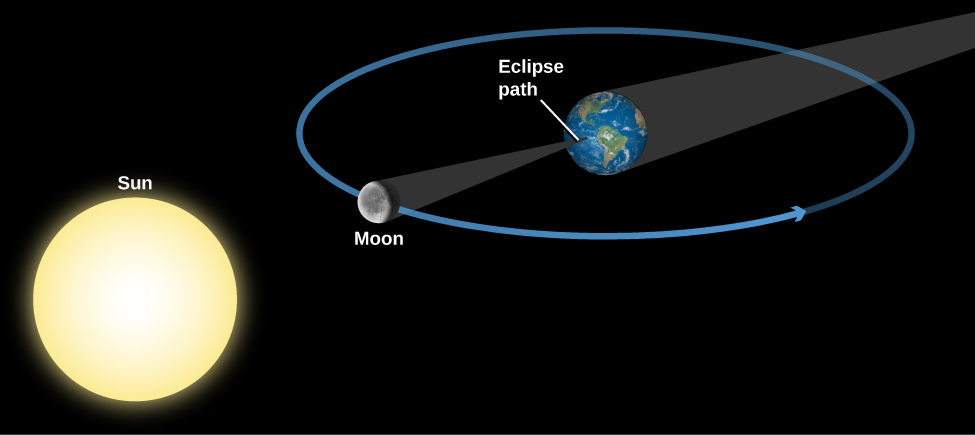
\includegraphics[width=2.5in]{Figures/Figure4.22.jpg}
\end{minipage}
\vspace{1em}

\question
Which part of the Sun may be seen during a solar eclipse? (Warning: never look directly at the Sun).

% \begin{choices}
%     \choice the core
%     \choice the photosphere
%     \choice the surface
%     \correctchoice the corona (outer atmosphere)
% \end{choices}

\question
How long does viewing a solar eclipse last?

\begin{choices}
    \choice about 1 hour
    \correctchoice no more than 7 minutes
    \choice 7 days
    \choice 1 month
\end{choices}

% \question
% Which phenomenon is represented in the figure below?
% \vspace{1em}

% \begin{minipage}{0.4\textwidth}
%     \centering
%     \begin{choices}
%     \correctchoice lunar eclipse
%     \choice supernova
%     \choice solar eclipse
%     \choice hypernova
%     \end{choices}
% \end{minipage}%
% \begin{minipage}{0.5\textwidth}
%     \centering
%     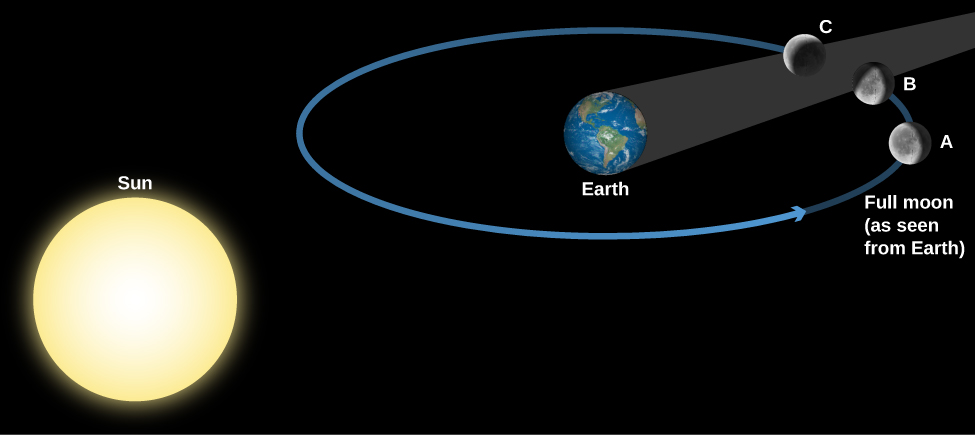
\includegraphics[width=3in]{Figures/Figure4.24.jpg}
% \end{minipage}

\clearpage
\question
What happens during a lunar eclipse?

\begin{choices}
    \choice The Moon blocks sunlight on Earth's surface.
    \choice The Moon's atmosphere reflects sunlight, turning it ``blood'' orange.
    \choice The Sun and Moon collide.
    \correctchoice The Earth blocks sunlight on the Moon's surface.
\end{choices}

\question
Why don't lunar and solar eclipses happen every month?

% \begin{choices}
%     \correctchoice The \SI{5}{\degree} tilt of the Moon's orbit usually prevents the Earth and Moon from crossing each others' shadows.
%     \choice The Sun isn't always bright enough to make eclipses happen.
%     \choice Eclipses only happen when at least 3 planets in the solar system align.
%     \choice They do happen every month; we just can't see them in Texas all the time.
% \end{choices}

\question 
What causes the Moon to turn ``blood'' orange during a lunar eclipse?

% \begin{choices}
%     \choice The Moon's atmosphere absorbs red wavelengths from the Sun.
%     \choice The Moon's true orange surface is made visible during an eclipse.
%     \correctchoice Earth's atmosphere focuses the redder wavelengths of light on the Moon (like during a sunset).
%     \choice The orange light from Mars reflects off the Moon
% \end{choices}

\question
Suppose it's been over 3 weeks since the last new moon. You look up at night and see the Moon below. What phase is this?

\begin{minipage}{0.3\textwidth}
    % \begin{choices}
    %     \choice waning gibbous
    %     \choice waxing gibbous
    %     \correctchoice waning crescent
    %     \choice waxing crescent
    % \end{choices}
\end{minipage}%
\begin{minipage}{0.3\textwidth}
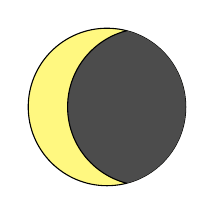
\begin{tikzpicture}
    \draw[fill=yellow!50] (0,0) circle (1cm);
    \begin{scope}
        \clip (0,0) circle (1cm);
        \draw[fill=black!70] (0.5,0) circle (1cm);
    \end{scope}
\end{tikzpicture}
\end{minipage}

\question
Suppose that a full moon will occur in a few days. You look up at night and see the Moon below. What phase is this?

\begin{minipage}{0.3\textwidth}
    % \begin{choices}
    %     \correctchoice waxing gibbous
    %     \choice waning gibbous
    %     \choice waxing crescent
    %     \choice waning crescent
    % \end{choices}
\end{minipage}%
\begin{minipage}{0.3\textwidth}
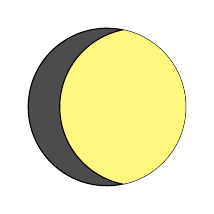
\begin{tikzpicture}
    \draw[fill=black!70] (0,0) circle (1cm);
    \begin{scope}
        \clip (0,0) circle (1cm);
        \draw[fill=yellow!50] (0.4,0) circle (1cm);
    \end{scope}
\end{tikzpicture}
\end{minipage}

\question
A perspective that is centered on Earth is \fillin\ .

\begin{choices}
\choice lunarcentric
\choice heliocentric
\correctchoice geocentric
\choice eccentric
\end{choices}


\question
What is the celestial sphere?

% \begin{choices}
% \correctchoice the apparent spherical shape of the sky
% \choice another name for the Sun
% \choice a nickname for Earth
% \choice A globe that shows the locations of countries
% \end{choices}

\question
Suppose you are outside viewing the night sky in Texas. Where is the zenith?

% \begin{choices}
% \choice on the horizon
% \choice below the horizon
% \choice on the Sun
% \correctchoice directly above you
% \end{choices}




\question
The \fillin\ is defined as the period of 1 revolution of Earth around the Sun.

\begin{choices}
\correctchoice year
\choice day
\choice month
\choice week
\end{choices}

\question
The Sun's path on the celestial sphere across the calendar year is called the \fillin\ .

% \begin{choices}
% \choice zodiac
% \choice constellation
% \choice solar path
% \correctchoice ecliptic
% \end{choices}

\question
The 13 constellations of the zodiac are aligned with \fillin \ .

\begin{minipage}{0.3\textwidth}
    \centering
    \begin{choices}
    \choice the north celestial pole
    \correctchoice the ecliptic
    \choice the zenith
    \choice the solar eclipse
    \end{choices}
\end{minipage}%
\begin{minipage}{0.6\textwidth}
    \centering
    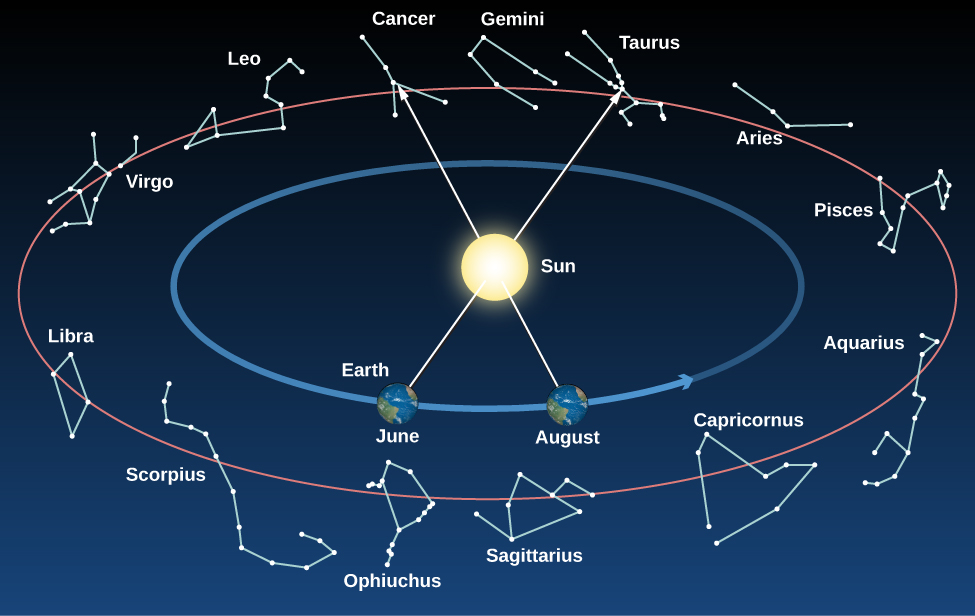
\includegraphics[width=0.5\textwidth]{Figures/Figure2.6.jpg}
\end{minipage}
\vspace{1em}

\question
What is the tilt of the celestial equator relative to the ecliptic?

\begin{minipage}{0.3\textwidth}
    \centering
    \begin{choices}
    \choice \SI{0.01}{\degree} 
    \choice \SI{30.0}{\degree} 
    \correctchoice \SI{23.5}{\degree} 
    \choice \SI{45.0}{\degree} 
    \end{choices}
\end{minipage}%
\begin{minipage}{0.6\textwidth}
    \centering
\scalebox{0.8}{
\centering
\begin{tikzpicture}

\def\R{3} % sphere radius
\def\angEl{23} % elevation angle
\def\angTilt{30} %tilt angle increased from 23.5 for emphasis

\pgfmathsetmacro\H{\R*cos(\angEl)} % distance to north pole
\draw (0,0) -- (0,\H*1.25);
\fill[yellow] (0.3,1.15) circle (3pt);
\draw[very thick] (0.3,1.15) circle (3pt);% node[above right] {\textbf{September}};

\begin{scope}[rotate=-\angTilt]
    \draw[very thin] (0,\H) -- (0,0);
\end{scope}
\shade[ball color=white, opacity=0.5] (0,0) circle (\R);
\coordinate[mark coordinate] (O) at (0,0);

\begin{scope}[rotate=-\angTilt]
    \DrawLatitudeCircleBack[\R]{0}
\end{scope}

\begin{scope}[rotate=-\angTilt]
        \DrawLatitudeCircleFront[\R]{0}
        \draw[thick] (0,\H*1.25) -- (0,\H) (0,0) -- (0,-1);
        \draw[very thick,blue,fill=white] (0,0) circle (19pt) node {\rotatebox{-\angTilt}{\textbf{Earth}}};
        \node at (0.2,0.9) {\textbf{N}};
        \node at (-0.2,-0.9) {\textbf{S}};
\end{scope}

\DrawLatitudeCircle[\R]{0}
\draw (-2,-0.9) --++ (-1.3,-0.6) node[below] {Ecliptic};

\fill[yellow] (-\R,0) circle (4pt); 
\draw[very thick] (-\R,0) circle (4pt);% node[left=7pt] {\textbf{December}};

\fill[yellow] (\R,0) circle (4pt);
\draw[very thick] (\R,0) circle (4pt);% node[right=6pt] {\textbf{June}};

\fill[yellow] (-0.3,-1.15) circle (4pt); 
\draw[very thick] (-0.3,-1.15) circle (4pt);% node[below=8pt] {\textbf{March}};

\draw[very thick,<->] (0,2.3) arc (90:55:1.85);
\node at (0.75,2.55) {tilt?};

\draw (1.7,-1.8) -- ++(1,-0.4) node[right] {Celestial Equator};

\draw[very thick,<->] (1.7,-1) arc (-10:-45:1.4);
\node at (2.1,-1.45) {\small {tilt?}};

\node at (-2.8,2.8) {Celestial Sphere};

\end{tikzpicture}
}
\end{minipage}
\vspace{1em}


\question
If a model is \textit{heliocentric}, then it is \fillin\ .

% \begin{choices}
% \choice centered on Earth
% \correctchoice centered on the Sun
% \choice centered on the Moon
% \choice ancient in origin
% \end{choices}



\question
Which shapes did Pythagoras believe to be ``perfect forms''?

% \begin{choices}
%     \choice hexagon
%     \choice rhombus \& rectangle
%     \choice ellipse
%     \correctchoice circle \& sphere
% \end{choices}

\question
Why did ancient Greeks like Pythagoras believe the gods prefer spheres?

% \begin{choices}
%     \choice the gods spoke to Pythagoras
%     \choice the human head is shaped like a sphere (ball)
%     \choice the gods actually preferred triangles
%     \correctchoice the Sun and Moon are round and spherical
% \end{choices}

\question
Which astronomical event did Aristotle reference to prove that the Sun must be farther away from us than the Moon?

% \begin{choices}
%     \choice a lunar eclipse
%     \choice the sun rise
%     \correctchoice a solar eclipse
%     \choice the blue moon
% \end{choices}

\question
Which of the following is NOT in agreement with Aristotle's arguments for a round Earth?

\begin{choices}
    \choice People in South America can see stars that are not visible in Texas.
    \choice The North Star looks lower in the sky in Florida than it does in Maine.
    \correctchoice The celestial sphere does not change when you geographically travel southward. 
    \choice Earth casts a round shadow on the Moon during a lunar eclipse.
\end{choices}


% \subsection*{Ptolemy's Model of the Solar System}

\question
Ptolemy's book, which served as the authority of astronomical knowledge for over 1400 years, was called the \fillin[\textit{Almagest}].

% \begin{choices}
%     \choice \textit{Principia Mathematica}
%     \correctchoice \textit{Almagest}
%     \choice \textit{On The Revolutions of Celestial Orbs}
%     \choice \textit{Harry Potter and the Chamber of Secrets}
% \end{choices}

\question
The purpose of Ptolemy's geometric model of the solar system was to \fillin\ .

% \begin{choices}
%     \choice prove that the solar system is geocentric
%     \choice create the 12 constellations of the zodiac
%     \correctchoice predict the positions of the Sun and planets at any date and time
%     \choice prove that the solar system is heliocentric
% \end{choices}

\question
True or False? Ptolemy's geocentric model was remarkable because it was simple and symmetrical.

\begin{choices}
    \choice True
    \correctchoice False
\end{choices}

% \clearpage
% \section*{2.4 The Birth of Modern Astronomy}

\question
What was Copernicus's motivation for challenging Ptolemy's model of the solar system?

\begin{choices}
    \choice He hated Ptolemy
    \correctchoice He wanted a better, simpler theory to predict where the planets will move in the sky
    \choice He wanted to prove that the geocentric model of the solar system was correct.
    \choice He actually agreed with Ptolemy's model.
\end{choices}

% \question
% What does ``heliocentric'' mean?

% \begin{choices}
%     \choice centered on the Earth
%     \choice centered on the Moon
%     \choice centered on Mars
%     \correctchoice centered on the Sun
% \end{choices}

\question
True or false? Ptolemy believed in a \textit{heliocentric} solar system, and Copernicus in a \textit{geocentric} one.

\begin{choices}
    \choice True
    \correctchoice False
\end{choices}

\question
According to Copernicus, the celestial sphere appears to rotate because\ldots\ .

% \begin{choices}
%     \correctchoice the Earth rotates on its axis (once every 24 hours)
%     \choice the Sun is the center of the solar system
%     \choice the universe revolves around the Earth
%     \choice the atmosphere creates a rotational effect
% \end{choices}

\question
True or False? Copernicus proved beyond doubt that Earth and the planets revolve around the Sun.

\begin{choices}
    \choice True
    \correctchoice False
\end{choices}

\question
True or False? Galileo was a supporter of the Copernican (sun-centered) view of the universe.

\begin{choices}
    \correctchoice True
    \choice False
\end{choices}

\question
What is the significance of the discovery of Jupiter's 4 moons?

% \begin{choices}
%     \choice It proved that the solar system is Earth-centered.
%     \choice It motivated Galileo to search the Milky Way for other faint objects.
%     \choice It supported the Church's stance on a heliocentric universe.
%     \correctchoice It was clear evidence that not everything revolves around Earth.
% \end{choices}

\question
After Galileo, Earth was \ldots

\begin{choices}
    \choice proven to be a round object
    \correctchoice no longer considered the center of the universe
    \choice considered to have 3 more moons
    \choice hit by an asteroid
\end{choices}

\question
Did Galileo face consequences for his astronomical observations?

\begin{choices}
    \choice No. He was hailed a hero.
    \choice No. No one cared about his experiments.
    \correctchoice Yes. He was put under house arrest. 
    \choice Yes. He was executed.
\end{choices}

\question
Wavelength is \fillin\ .

% \begin{choices}
%     \choice the vertical distance between neighboring crests in a wave
%     \choice the distance between a crest and a trough in a wave
%     \choice the distance traveled by a wave in 1 second 
%     \correctchoice the horizontal distance between neighboring crests in a wave
% \end{choices}

\question
What is a wave cycle?

\begin{choices}
    \correctchoice the portion of a wave encompassed by 1 wavelength
    \choice the distance from a crest to a trough
    \choice a series of waves in the ocean
    \choice the time it takes a wave to vibrate
\end{choices}

\question
How many wave cycles are shown below?

\begin{figure}[h!]
    \centering
    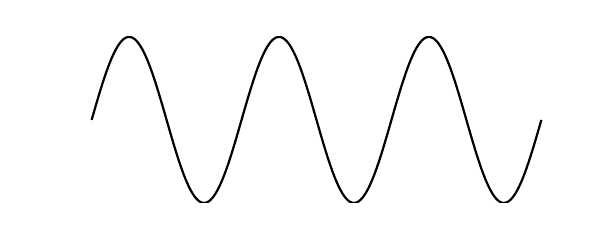
\begin{tikzpicture}
    \def\waveStart{0} %pi/2, pi, 3*pi/2, 0
    \def\nWaves{3}
    \begin{axis}[width=240pt,height=105pt,
        yticklabels={,,},
        xticklabels={,,},
        axis line style={draw=none},
        tick style={draw=none},   
        ymin=-1,
        ymax=1,
    ]
    \addplot[thick, color=black,
        domain=\waveStart:\waveStart+2*pi*\nWaves,
        samples=250]
        {sin(deg((x))};
    \end{axis}
    \end{tikzpicture}
\end{figure}

\begin{oneparchoices}
    \choice 3.5
    \correctchoice 3
    \choice 7
    \choice 6
\end{oneparchoices}

% \question
% How many wave cycles are shown below?
% \begin{figure}[h!]
%     \centering
%     \begin{tikzpicture}
%     \def\waveStart{pi} %pi/2, pi, 3*pi/2, 0
%     \def\nWaves{6.5}
%     \begin{axis}[width=360pt,height=105pt,
%         yticklabels={,,},
%         xticklabels={,,},
%         axis line style={draw=none},
%         tick style={draw=none},   
%         ymin=-1,
%         ymax=1,
%     ]
%     \addplot[thick, color=black,
%         domain=\waveStart:\waveStart+2*pi*\nWaves,
%         samples=250]
%         {sin(deg((x))};
%     \end{axis}
%     \end{tikzpicture}
% \end{figure}

% \begin{oneparchoices}
%     \choice 6
%     \choice 12
%     \correctchoice 6.5
%     \choice 13
% \end{oneparchoices}

\question
What is electromagnetic radiation?

% \begin{choices}
%     \choice the portion of a wave encompassed by 1 wave cycle
%     \choice toxic gases that travel in waves through the air
%     \choice electrons moving through a magnetic field
%     \correctchoice waves of combined electric and magnetic fields moving at light-speed
% \end{choices}

\question
What is a photon?

% \begin{choices}
%     \choice a small portion of an electromagnetic wave
%     \choice a subatomic particle in the nucleus 
%     \correctchoice a particle of light; a unit of electromagnetic radiation
%     \choice the uppermost part of a wave
% \end{choices}

\question
What are the seven regions of the electromagnetic spectrum?

% \begin{choices}
%     \choice red, orange, yellow, green, blue, indigo, violet
%     \correctchoice radio, microwave, infrared, visible light, ultraviolet, X-ray, gamma ray
%     \choice radio, microwave, infrared, green, blue, indigo, violet
%     \choice red, orange, yellow, green, ultraviolet, X-ray, gamma ray
% \end{choices}

\question
Which type of electromagnetic wave has the \textit{highest} energy?

% \begin{choices}
%     \choice visible light
%     \choice radio
%     \choice X-ray
%     \correctchoice gamma ray
% \end{choices}

\question
Which type of electromagnetic wave has the \textit{lowest} energy?

\begin{choices}
    \choice ultraviolet
    \correctchoice radio
    \choice microwaves
    \choice infrared
\end{choices}

% \question
% What is the range of wavelength, in nanometers (nm), for visible light?

% \begin{choices}
%     \choice 0.01--\SI{20}{nm}
%     \choice $10^6$--$10^9\,$nm
%     \correctchoice 400--\SI{700}{nm}
%     \choice 20--\SI{400}{nm}
% \end{choices}

% \question
% The frequency of an electromagnetic wave is given by the equation below:

% \begin{equation*}
%     f = \frac{c}{\lambda}\ ,
% \end{equation*}

% where $c = \SI{3e8}{m/s}$ is the speed of light and $\lambda$ is wavelength in meters. What is the frequency of a green light wave with a wavelength of \SI{525}{nm}? (Note: \SI{1}{nm} = \SI{1e-9}{m}.) 
% \textit{Tip}: Use \href{https://www.desmos.com/scientific}{desmos.com/scientific}

\question
What do we see when telescopic instruments capture the Sun in wavelengths outside of the visible light portion of the spectrum, like in X-ray, ultraviolet, or infrared?

\begin{choices}
    \choice Nothing; the Sun is not visible outside the visible portion of the spectrum
    \choice the Sun's rings become apparent
    \choice The true color of the Sun is green
    \correctchoice New parts of the Sun that are normally not visible in normal photographs
\end{choices}

\question
What did Newton discover about sunlight using the apparatus below?

\begin{figure}[h!]
    \centering
    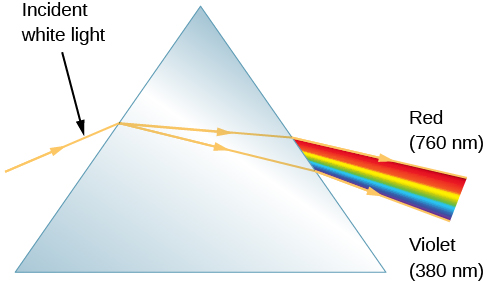
\includegraphics[width=2in]{Figures/Figure5.9.jpg}
\end{figure}

\begin{choices}
    \correctchoice sunlight is made of the colors of the the rainbow
    \choice sunlight contains infrared light
    \choice some colors are warmer than others
    \choice the spectrum contains dark vertical lines
\end{choices}

\question
The figure below is the spectrum of the Sun. What causes the dark lines?

\begin{figure}[h!]
    \centering
    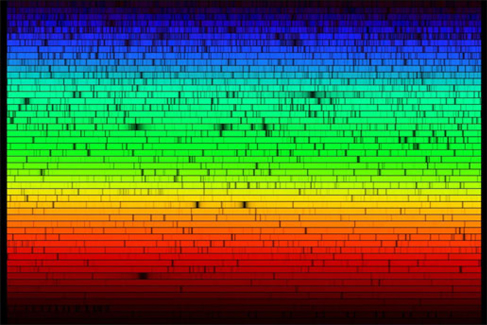
\includegraphics[width=2.5in]{Figures/Figure5.11.jpg}
\end{figure}

\begin{choices}
    \choice imperfections in the manufacturing of the prism
    \choice Earth's atmosphere 
    \choice infrared light waves
    \correctchoice atoms in the Sun absorbing particular wavelengths of light
\end{choices}

% \question
% Jules Janssen was the first to observe the presence of helium in the Sun. The yellow spectral line for helium was very close to the sodium doublet lines. What is the approximate wavelength of these lines, in nanometers?

% \begin{choices}
%     \choice \SI{100}{nm}
%     \choice \SI{325}{nm}
%     \correctchoice \SI{589}{nm}
%     \choice \SI{700}{nm}
% \end{choices}

\question
How do we know what the Sun is made of?

\begin{choices}
    \choice We collect samples and bring them back to Earth.
    \choice We capture its light and see what the light is made of.
    \choice We actually don't know what the Sun is made of.
    \correctchoice We analyze the absorption lines in its spectrum.
\end{choices}

% \question
% In what year was Tycho Brahe born?

% \begin{choices}
%     \choice 1609
%     \choice 1543
%     \choice 1776
%     \correctchoice 1546
% \end{choices}

\question
What was Tycho Brahe's greatest contribution to astronomy?

\begin{choices}
    \choice He discovered and wrote the 3 laws of planetary motion.
    \choice He was a gifted mathematician who developed of Law of Universal Gravitation.
    \correctchoice He made excellent measurements of solar and planetary positions for 20 years. 
    \choice He observed the Moon and planets with a telescope.
\end{choices}

% \question
% True or False? Tycho Brahe was skilled at using a telescope to record planetary motions.

% \begin{choices}
%     \choice True
%     \correctchoice False
% \end{choices}

% \question
% What prevented Brahe from creating a better model of planetary motion than Ptolemy's ancient model?

\question
Who did Brahe hire to analyze his data?

\begin{choices}
    \choice Isaac Newton
    \choice Galileo Galilei
    \choice Thomas Jefferson
    \correctchoice Johannes Kepler
\end{choices}

% \question
% In what year was Johannes Kepler born?

% \begin{choices}
%     \choice 1609
%     \choice 1546
%     \choice 1630
%     \correctchoice 1571
% \end{choices}

% \question
% Kepler studied \fillin[theology] at the University of Tubingen.

% \begin{choices}
%     \correctchoice theology 
%     \choice biology
%     \choice chemistry
%     \choice anatomy
% \end{choices}

\question
What idea or system did Kepler encounter during his time in the university?

\begin{choices}
    \choice Newton's Law of Universal Gravitation.
    \choice The 3 Laws of Planetary Motion.
    \choice Darwin's theory of evolution.
    \correctchoice Copernicus's heliocentric (Sun-centered) hypothesis of the solar system.
\end{choices}

% \question
% Who hired Kepler? For what purpose was Kepler hired?

\question
What did Kepler inherit from Brahe?

\begin{choices}
    \choice A lot of money.
    \choice His observatory.
    \correctchoice Two decades' worth of accurate data on planetary positions in the sky. 
    \choice A manual on how to use the telescope for astronomical observation.
\end{choices}

\question
What is an orbit?

\begin{choices}
    \choice the amount of time it takes a planet to go around the Sun
    \choice the distance between the Sun and a planet
    \correctchoice the path a planet takes around the Sun
    \choice the Houston Astros mascot
\end{choices}

\question
Initially Kepler assumed the shape of a planet's orbit was \fillin\ .

\begin{choices}
    \correctchoice a circle
    \choice an ellipse
    \choice a parabola
    \choice a square
\end{choices}

\question
What made Kepler change his mind about his original assumption of the shape of orbits?

\begin{choices}
    \choice Brahe explained to him the correct answer. 
    \choice He read about it in Copernicus's book.
    \correctchoice The shape of the orbit of Mars refuted his hypothesis.
    \choice He had a dream in which angels revealed to him the truth.
\end{choices}

\question
What is an ellipse?

\begin{choices}
    \choice a perfect circle
    \correctchoice a flattened circle
    \choice when the Moon blocks the Sun (or vice-versa)
    \choice a flattened square
\end{choices}

\question
Kepler's First Law of motion states the shape of the orbit of a planet is \fillin\ .

\begin{choices}
    \correctchoice an ellipse 
    \choice a circle
    \choice a rectangle
    \choice a triangle
\end{choices}


% \question
% Kepler's Second Law of Motion
% states that when a planet is closer to the Sun, it moves \fillin[faster], and when it's farther away, it
% moves \fillin[slower], but it sweeps out equal areas in an equal times.

% \question
% What is Kepler's Third Law of Motion?

% \begin{choices}
%     \choice Every action has an equal and opposite reaction.
%     \choice Net force equals mass times acceleration ($F_{\text{net}} = m a$)
%     \correctchoice Orbital period squared is proportional to semimajor axis cubed ($P^2 \propto a^3$)
%     \choice The square of the hypotenuse equals the sum of the square of sides ($a^2 + b^2 = c^2$).
% \end{choices}

% \question
% In Kepler's Third Law, what does the $P$ stand for? What units should be used?

% \question
% In Kepler's Third Law, what does the $a$ stand for? What units should be used?

\question
Saturn has a semimajor axis of \SI{9.54}{AU}. What is Saturn's orbital period? (\textit{Hint}: Use Kepler's 3rd Law of Motion: $P = \sqrt{a^3}$\,).

\begin{choices}
    \choice \SI{11.8}{yr}
    \choice \SI{27.65}{yr}
    \correctchoice \SI{29.46}{yr}
    \choice \SI{84.5}{yr}
\end{choices}

\question
Identify the constellation below.

\begin{minipage}{0.3\textwidth}
\centering
    \begin{choices}
        \choice %Scorpius
        \correctchoice %Orion
        \choice %Ursa Major
        \choice %Taurus
    \end{choices}
\end{minipage}%
\begin{minipage}{0.5\textwidth}
    \centering
    % 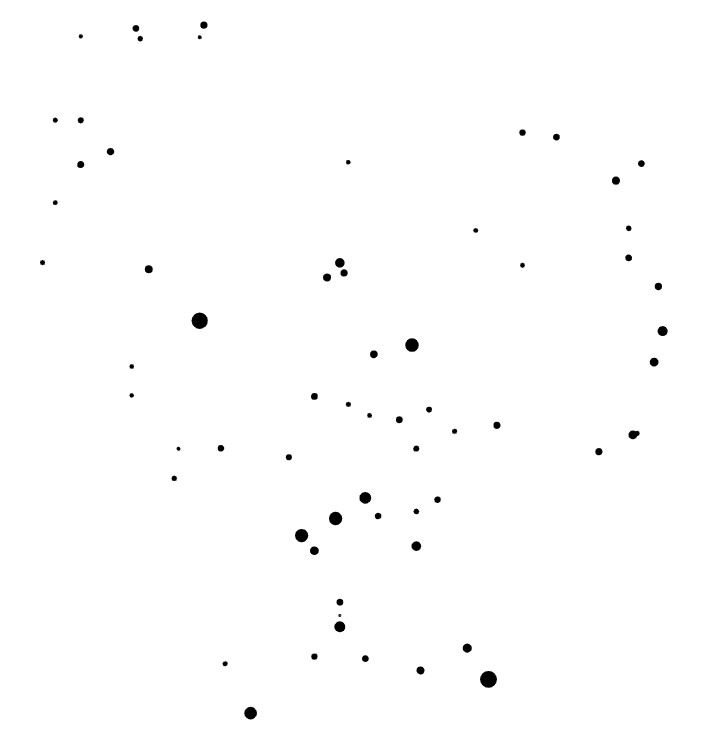
\includegraphics[width=5cm]{Figures/OrionConst.png}
\begin{tikzpicture}
\begin{axis}[%
    height=7cm, width=7cm,
    x dir=reverse,
    axis line style={draw=none},
    ticks=none,
]
\addplot[%
    scatter=true,
    only marks,
    mark=*,
    point meta=explicit symbolic,
    scatter/@pre marker code/.style={/tikz/mark size=\pgfplotspointmeta/4},
    scatter/@post marker code/.style={}
] table [meta index=2] {Unit6_Constellations/Constellations/Orion.dat};

\iftoggle{printstars}{
\node[right=2pt] at (5.24,-8.20) {\footnotesize Rigel};
\node[left=2pt] at (5.92,7.41) {\footnotesize Betelgeuse};
}{}

\iftoggle{printlines}{
\draw
(6.06,19.69) --
(6.20,14.21) --
(6.13,14.77)
(6.20,14.21) --
(6.04,9.65)
(5.91,20.28) --
(6.13,14.77) --
(6.04,9.65) --
(5.92,7.41) --
(5.68,-1.94) --
(5.60,-1.20) --
(5.53,-0.30)
(5.68,-1.94) --
(5.80,-9.67) --
(5.24,-8.20) --
(5.53,-0.30) --
(5.42,6.35) -- % Bellatrix
(5.59,9.93) --
(5.92,7.41)
(5.42,6.35) --
(4.83,6.96) % Tabit
(4.91,10.15) --
(4.84,8.90) --
(4.83,6.96) --% Tabit
(4.85,5.61) --
(4.90,2.44) --
(4.98,1.71)
;

}{}
\end{axis}
\end{tikzpicture}
\end{minipage}

\question
Identify the constellation below.

\begin{minipage}{0.3\textwidth}
\centering
    \begin{choices}
        \choice %
        \choice %
        \choice %
        \choice %
    \end{choices}
\end{minipage}%
\begin{minipage}{0.5\textwidth}
    \centering
\begin{tikzpicture}
\begin{axis}[%
    height=7cm, width=7cm,
    x dir=reverse,
    axis line style={draw=none},
    ticks=none,
]
\addplot[%
    scatter=true,
    only marks,
    mark=*,
    point meta=explicit symbolic,
    scatter/@pre marker code/.style={/tikz/mark size=\pgfplotspointmeta/4},
    scatter/@post marker code/.style={}
] table [meta index=2] {Unit6_Constellations/Constellations/Scorpius.dat};

\iftoggle{printstars}{
\node[below right=-2pt] at (16.49,-26.43) {\footnotesize Antares};
}{}

\iftoggle{printlines}{
\draw
(17.56,-37.10) -- % Shaula
(17.71,-39.03) --
(17.79,-40.13) --
(17.62,-43.00) -- % Sargas
(17.20,-43.24) --
(16.91,-42.36) -- % Grafias
(16.87,-38.02) --
(16.84,-34.29) --
(16.60,-28.22) -- % Alniyat
(16.49,-26.43) -- % Antares
(16.09,-19.81) % Acrab
(16.49,-26.43) -- % Antares
(16.01,-22.62) % Dschubba
(16.49,-26.43) -- % Antares
(15.98,-26.11)
;
}{}
\end{axis}
\end{tikzpicture}
\end{minipage}

\question 
Identify the constellation below.

\begin{minipage}{0.3\textwidth}
\centering
    \begin{choices}
        \choice %
        \choice %
        \choice %
        \choice %
    \end{choices}
\end{minipage}%
\begin{minipage}{0.5\textwidth}
    \centering
\begin{tikzpicture}
\begin{axis}[%
    height=7cm, width=7cm,
    x dir=reverse,
    axis line style={draw=none},
    ticks=none,
]
\addplot[%
    scatter=true,
    only marks,
    mark=*,
    point meta=explicit symbolic,
    scatter/@pre marker code/.style={/tikz/mark size=\pgfplotspointmeta/4},
    scatter/@post marker code/.style={}
] table [meta index=2] {Unit6_Constellations/Constellations/UrsaMinor.dat};


\node[right=2pt] at (17.94,89.9) {\footnotesize The North Star};


\iftoggle{printlines}{
\draw
(17.94,89.9) -- % Polaris. Coordinates modified to fit plot.
(17.54,86.59) -- 
(16.77,82.04) --
(15.73,77.79) -- 
(14.85,74.16) -- % Kochab
(15.35,71.83) -- 
(16.18,75.88) -- 
(15.73,77.79);
}{}
\end{axis}
\end{tikzpicture}
\end{minipage}

\question 
Identify the constellation below.

\begin{minipage}{0.3\textwidth}
\centering
    \begin{choices}
        \choice %
        \choice %
        \choice %
        \choice %
    \end{choices}
\end{minipage}%
\begin{minipage}{0.5\textwidth}
    \centering
\begin{tikzpicture}
\begin{axis}[%
    height=7cm, width=7cm,
    x dir=reverse,
    axis line style={draw=none},
    ticks=none,
]
\addplot[%
    scatter=true,
    only marks,
    mark=*,
    point meta=explicit symbolic,
    scatter/@pre marker code/.style={/tikz/mark size=\pgfplotspointmeta/4},
    scatter/@post marker code/.style={}
] table [meta index=2] {Unit6_Constellations/Constellations/UrsaMajor.dat};

\iftoggle{printstars}{
\node[below right=-2pt] at (13.40,54.93) {\footnotesize Mizar};
}{}

\iftoggle{printlines}{
\draw
(13.79,49.31) -- % Alkaid
(13.40,54.93) -- % Mizar
(12.90,55.96) -- % Alioth
(12.26,57.03) -- % Megrez
(11.90,53.69) -- % Phad
(11.77,47.78) -- 
(11.16,44.50) --
(10.37,41.50)
(11.16,44.50) --
(10.28,42.91)
(12.26,57.03) -- % Megrez
(11.06,61.75) -- % Dubhe
(11.03,56.38) % Merak
(11.06,61.75) -- % Dubhe
(9.53,63.06) -- 
(8.50,60.72) --
(9.85,59.04) --
(9.87,54.06) -- %
(9.55,51.68) --
(9.06,47.16)
(9.55,51.68) --
(8.99,48.04)
(11.90,53.69) -- % Phad
(11.03,56.38) -- % Merak
(9.87,54.06);
}{}
\end{axis}
\end{tikzpicture}
\end{minipage}

\end{questions}
\end{document}



